%-------------------------------------------------------------------------------------------------%
\documentclass[12pt]{article}

%-------------------------------------------------------------------------------------------------%
\usepackage[spanish]{babel}
\usepackage[margin=1in]{geometry}
\usepackage[hidelinks]{hyperref}
\usepackage{amssymb,amsmath,amsthm,amsfonts}
\usepackage{enumerate}
\usepackage{graphicx}
\usepackage{datetime}
\usepackage{parskip}
\usepackage{apacite}
\usepackage{lipsum}
\usepackage{color}
\usepackage{float}
\usepackage{cancel}
%-------------------------------------------------------------------------------------------------%
\newenvironment{solution}{\begin{proof}[Solución]}{\end{proof}}
\renewcommand{\qedsymbol}{\rule{0.7em}{0.7em}}
\newtheorem{proposition}{Proposición}
\newtheorem{observation}{Observación}
\newtheorem{afirmation}{Afirmación}
\newtheorem{definition}{Definición}
\newtheorem{corollary}{Corolario}
\newtheorem{exercise}{Ejercicio}
\newtheorem{theorem}{Teorema}
\newtheorem{example}{Ejemplo}
\newtheorem{lemma}{Lema}
\graphicspath{{Img/}}
\decimalpoint
%-------------------------------------------------------------------------------------------------%
\title{Tarea 4 - Optimización No Lineal}
\author{Camara Medina Cynthia Lilian \\
Reyes Zamora Ollin \\
Alanis González Edzon Omar \\[0.2cm]
Mendoza Urrusquieta Jair Natael}
\date{\today}
%-------------------------------------------------------------------------------------------------%
\makeatletter
\let\thetitle\@title
\let\theauthor\@author
\let\thedate\@date
\makeatother
%-------------------------------------------------------------------------------------------------%
\begin{document}
%-------------------------------------------------------------------------------------------------%
\begin{titlepage}
\centering

\includegraphics[width=0.9\linewidth]{logo.png}\\[2.0 cm]
\textsc{\LARGE Escuela Superior de Física y Matemáticas}\\[1.2 cm]
\textsc{\Large Instituto Politécnico Nacional}\\[2.5 cm]
\rule{\linewidth}{0.2 mm} \\[0.4 cm]
{\huge \bfseries \thetitle}\\
\rule{\linewidth}{0.2 mm} \\[2.5 cm]
\textsc{\large \theauthor}
\vfill
{\large \thedate}
\end{titlepage}
%-------------------------------------------------------------------------------------------------%

\section*{Preguntas}

\begin{enumerate}
    \item \textbf{¿Cuál es la importancia de la condición de Armijo vista en clase?}
    
    Que es una técnica unidireccional muy efectiva, puesto que imponemos una condición que disminuye a la función objetivo, cumpliendo la condición de suficiencia.

		En este caso el decremento es definido a través de una desigualdad muy sencilla:
		\[f(x_k+\alpha v_k)\leq f(x_k)+C_1\alpha \bigtriangledown f_k^Tv_k\]
    \item \textbf{¿Por qué es importante la condición de curvatura de Wolfe? ¿es necesaria siempre? Explique.}
    
    La condición de curvatura de Wolfe no siempre es necesaria, y ¿por qué no siempre es necesaria?
		Como sabemos la condición de Armijo impone cotas a cuan grande puede ser el paso en la dirección "$v_k$" . Sin embargo, puede ocurrir que el paso sea tan pequeño que  $x_k$  no converja a un mínimo local.

		Ahí es donde entra una segunda condición la cual llamamos "Condición de Curvatura de Wolfe", la cual consiste prácticamente en acotar inferiormente a x.
		
		La podemos expresar de la siguiente manera:

			\[\bigtriangledown f(x_k+\alpha_kV_k)^T\geq C_2\bigtriangledown f_k^TV_k\]
		
		En conclusión, es de suma importancia en los casos donde la primera condición (Armijo) de pasos muy cortos y no converge, si converge con la primera condición, entonces no es necesaria la Condición de Curvatura de Wolfe.
    \item \textbf{Enumere las posibles desventajas del método de Newton para resolver problemas de optimización con varias variables.}
    
    \begin{itemize}
        \item Resolver el sistema de ecuaciones igualados a cero.
        \item Calcular las derivadas de las funciones objetivos una vez ya derivada.
        \item El número de llamados y evaluaciones a la función.
    \end{itemize}
    \item \textbf{Explique cuál es la razón de que existan modificaciones al método de Newton para optimización.}
    
    Los métodos usando la dirección de Newton son muy rápidos pero costosos puesto que hay que calcular y almacenar el hessiano. En ocasiones no es adecuado elegir un valor cercano al óptimo, pues la búsqueda lineal que nos brinda el método de Newton es muy larga y realmente sólo estamos interesados en reducir el valor de la función. Además, es bien conocido que este método, en general diverge violentamente. Es por ello que surgieron variantes como los métodos globalmente convergentes que tienen las propiedades del método de Newton en un entorno del punto.
    \item \textbf{Dada una matriz simétrica, explique cómo se puede determinar si esta es o no definida positiva.}
    
    Diremos qu una matriz es definida positiva  si y sólo si, todos los valores propios de la matriz $Q(z)$ son positivos y la definimos como negativa si y solo si, todos los valores propios de la matriz $Q(z)$ son negativas.
		
		Todo esto solo para matices cuadráticas o simétricas.
		
		Es decir la matriz cuadrática está definida de la forma: $Q(z)= z^t \cdot Q \cdot z$
\end{enumerate}


\section*{Búsqueda unidireccional inexacta}

\begin{enumerate}
    \item Minimizar \[f(x_1,x_2) = 8x_1^2 + 4x_1x_2 + 5x_2^2\] con $x^0 = [10,10]^T$.
    \begin{figure}[H]
        \centering
        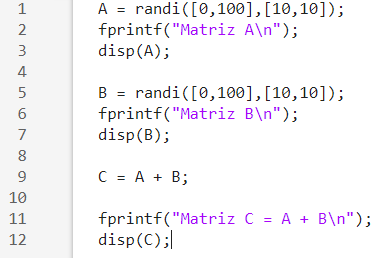
\includegraphics[height = 150px]{figura1.png}
    \end{figure}
    \item Minimizar \[f(x_1,x_2) = 2x_1^3+4x_1x_2^3-10x_1x_2+x_2^2\] con $x^0 = [5,2]^T$.
    \begin{figure}[H]
      \centering
      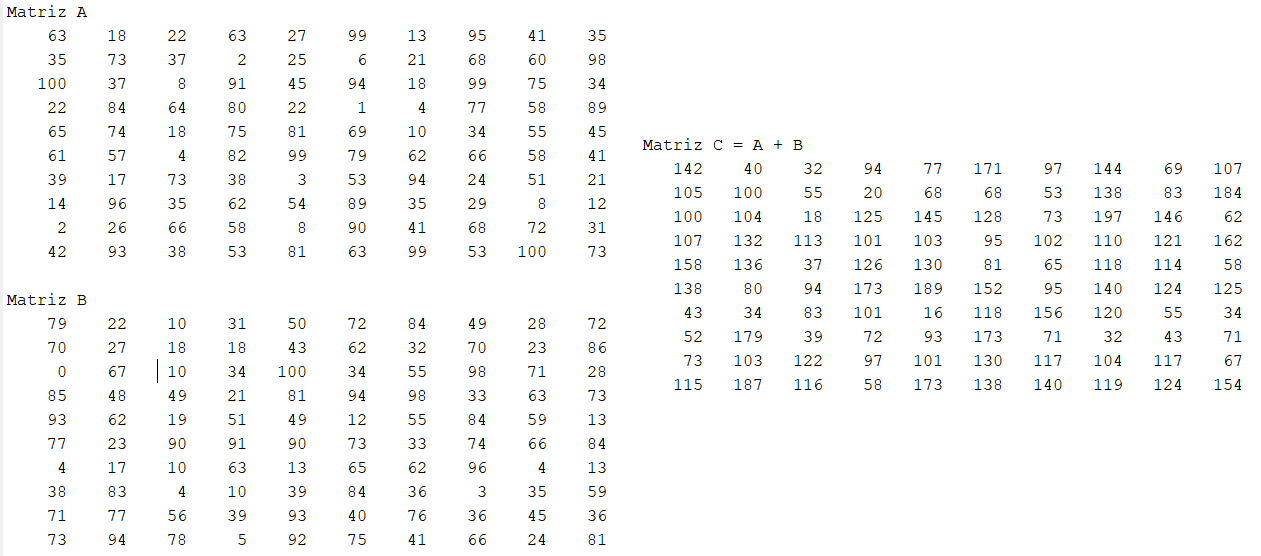
\includegraphics[height = 150px]{figura2.png}
  \end{figure}
  \newpage
    \item Minimizar \[f(x,y) = 2x^2-1.05x^4 + \frac{x^6}{6} + xy + y^2\] elija el punto inicial.
    \begin{figure}[H]
      \centering
      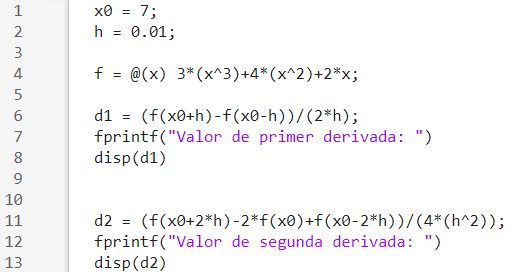
\includegraphics[height = 150px]{figura3.png}
  \end{figure}

  \vfill{}

    \item Minimizar \[f(x,y) = (x+2y-7)^2+(2x+y-5)^2\] elija el punto inicial.
    \begin{figure}[H]
      \centering
      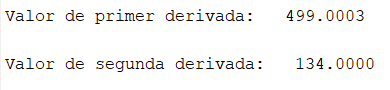
\includegraphics[height = 150px]{figura4.png}
  \end{figure}
\end{enumerate}

\vfill{}

\subsection*{Notas}

Nota 1: Para el método de Newton en la 2° función a minimizar se propuso un intervalo adicional dado que con el intervalo dado se llegaba a un punto silla.

Nota 2: Para la condición de Armijo empleamos el método de Newton para obtener el primer valor de $\alpha$. 

\newpage

\subsection*{Conclusiones}

Observamos que este método realiza muchas más iteraciones para hallar el valor de alpha que los otros dos métodos lo que hace que emplee más tiempo para llegar a una buena aproximación a pesar de disminuir la precisión (a comparación de los otros dos métodos). La condición de Armijo es más eficiente mientras más cerca esté el punto inicial del valor óptimo.

Desde nuestro punto de vista, el método más eficiente es el método de Newton.



\section*{Bibliografía}

\begin{itemize}
  \item D.G. LUENBERGER : Programación lineal y no lineal. AddisonWesley Iberoamericana, 1989.
  \item F. BONNANS - J. Ch. GILBERT - C. LEMARECHAL - C. SAGASTIZABAL : Optimisation Numérique: aspects théoriques et pratiques.
  SMAI-Springer Verlag, 1997.
  \item R. FLETCHER : Practical Methods of Optimization. Wiley, 1987.
  \item "Programación lineal y métodos de optimización", Eduardo Ramos Méndez, Universidad Nacional de Educación a Distancia. Madrid. 1997.
\end{itemize}

%-------------------------------------------------------------------------------------------------%
\end{document}
%-------------------------------------------------------------------------------------------------%